\documentclass[cjk,dvipdfmx,12pt,%
hyperref={bookmarks=true,bookmarksnumbered=true,bookmarksopen=false,%
colorlinks=false,%
pdftitle={第 50 回 関西 Debian 勉強会},%
pdfauthor={倉敷・のがた・佐々木},%
%pdfinstitute={関西 Debian 勉強会},%
pdfsubject={資料},%
}]{beamer}

\title{第 50 回 関西 Debian 勉強会}
\subtitle{{\scriptsize 資料}}
\author[倉敷 悟]{{\large\bf 倉敷・のがた・佐々木}}
\institute[Debian JP]{{\normalsize\tt 関西 Debian 勉強会}}
\date{{\small 2011 年 8 月 28 日}}

%\usepackage{amsmath}
%\usepackage{amssymb}
\usepackage{graphicx}
\usepackage{moreverb}
\usepackage[varg]{txfonts}
\AtBeginDvi{\special{pdf:tounicode EUC-UCS2}}
\AtBeginSection[]{\begin{frame}<beamer>\frametitle{Agenda}\tableofcontents[currentsection]\end{frame}}
\usetheme{Kyoto}
\def\museincludegraphics{%
  \begingroup
  \catcode`\|=0
  \catcode`\\=12
  \catcode`\#=12
  \includegraphics[width=0.9\textwidth]}
%\renewcommand{\familydefault}{\sfdefault}
%\renewcommand{\kanjifamilydefault}{\sfdefault}
\begin{document}
\settitleslide
\begin{frame}
\titlepage
\end{frame}
\setdefaultslide

\begin{frame}[fragile]
\frametitle{Agenda}
\tableofcontents
\end{frame}

\begin{frame}[fragile]
\frametitle{ところで}

今日の宴会ってドコなの?

\end{frame}

\section{最近の Debian 関係のイベント}

\takahashi[40]{最近の Debian\\関係のイベント}

\begin{frame}[fragile]
\frametitle{OSC 2011 Kyoto}

\begin{itemize}
\item 日時: 7 月 16 日
\item 於: OSC 2011 Kyoto, 京都リサーチパーク
\end{itemize}

\begin{block}{内容}
  \begin{itemize}
  \item Debian, squeeze, Wheezy, and Sid by 佐々木
  \end{itemize}
\end{block}
\end{frame}

\begin{frame}[fragile]
  \frametitle{Debconf11}
  \begin{itemize}
  \item 2011/07/24 -- 30
  \item 於: ボスニア
  \item 東京エリアの岩松さん, やまねさん, 野島さんが参加
  \end{itemize}
  \begin{center}
    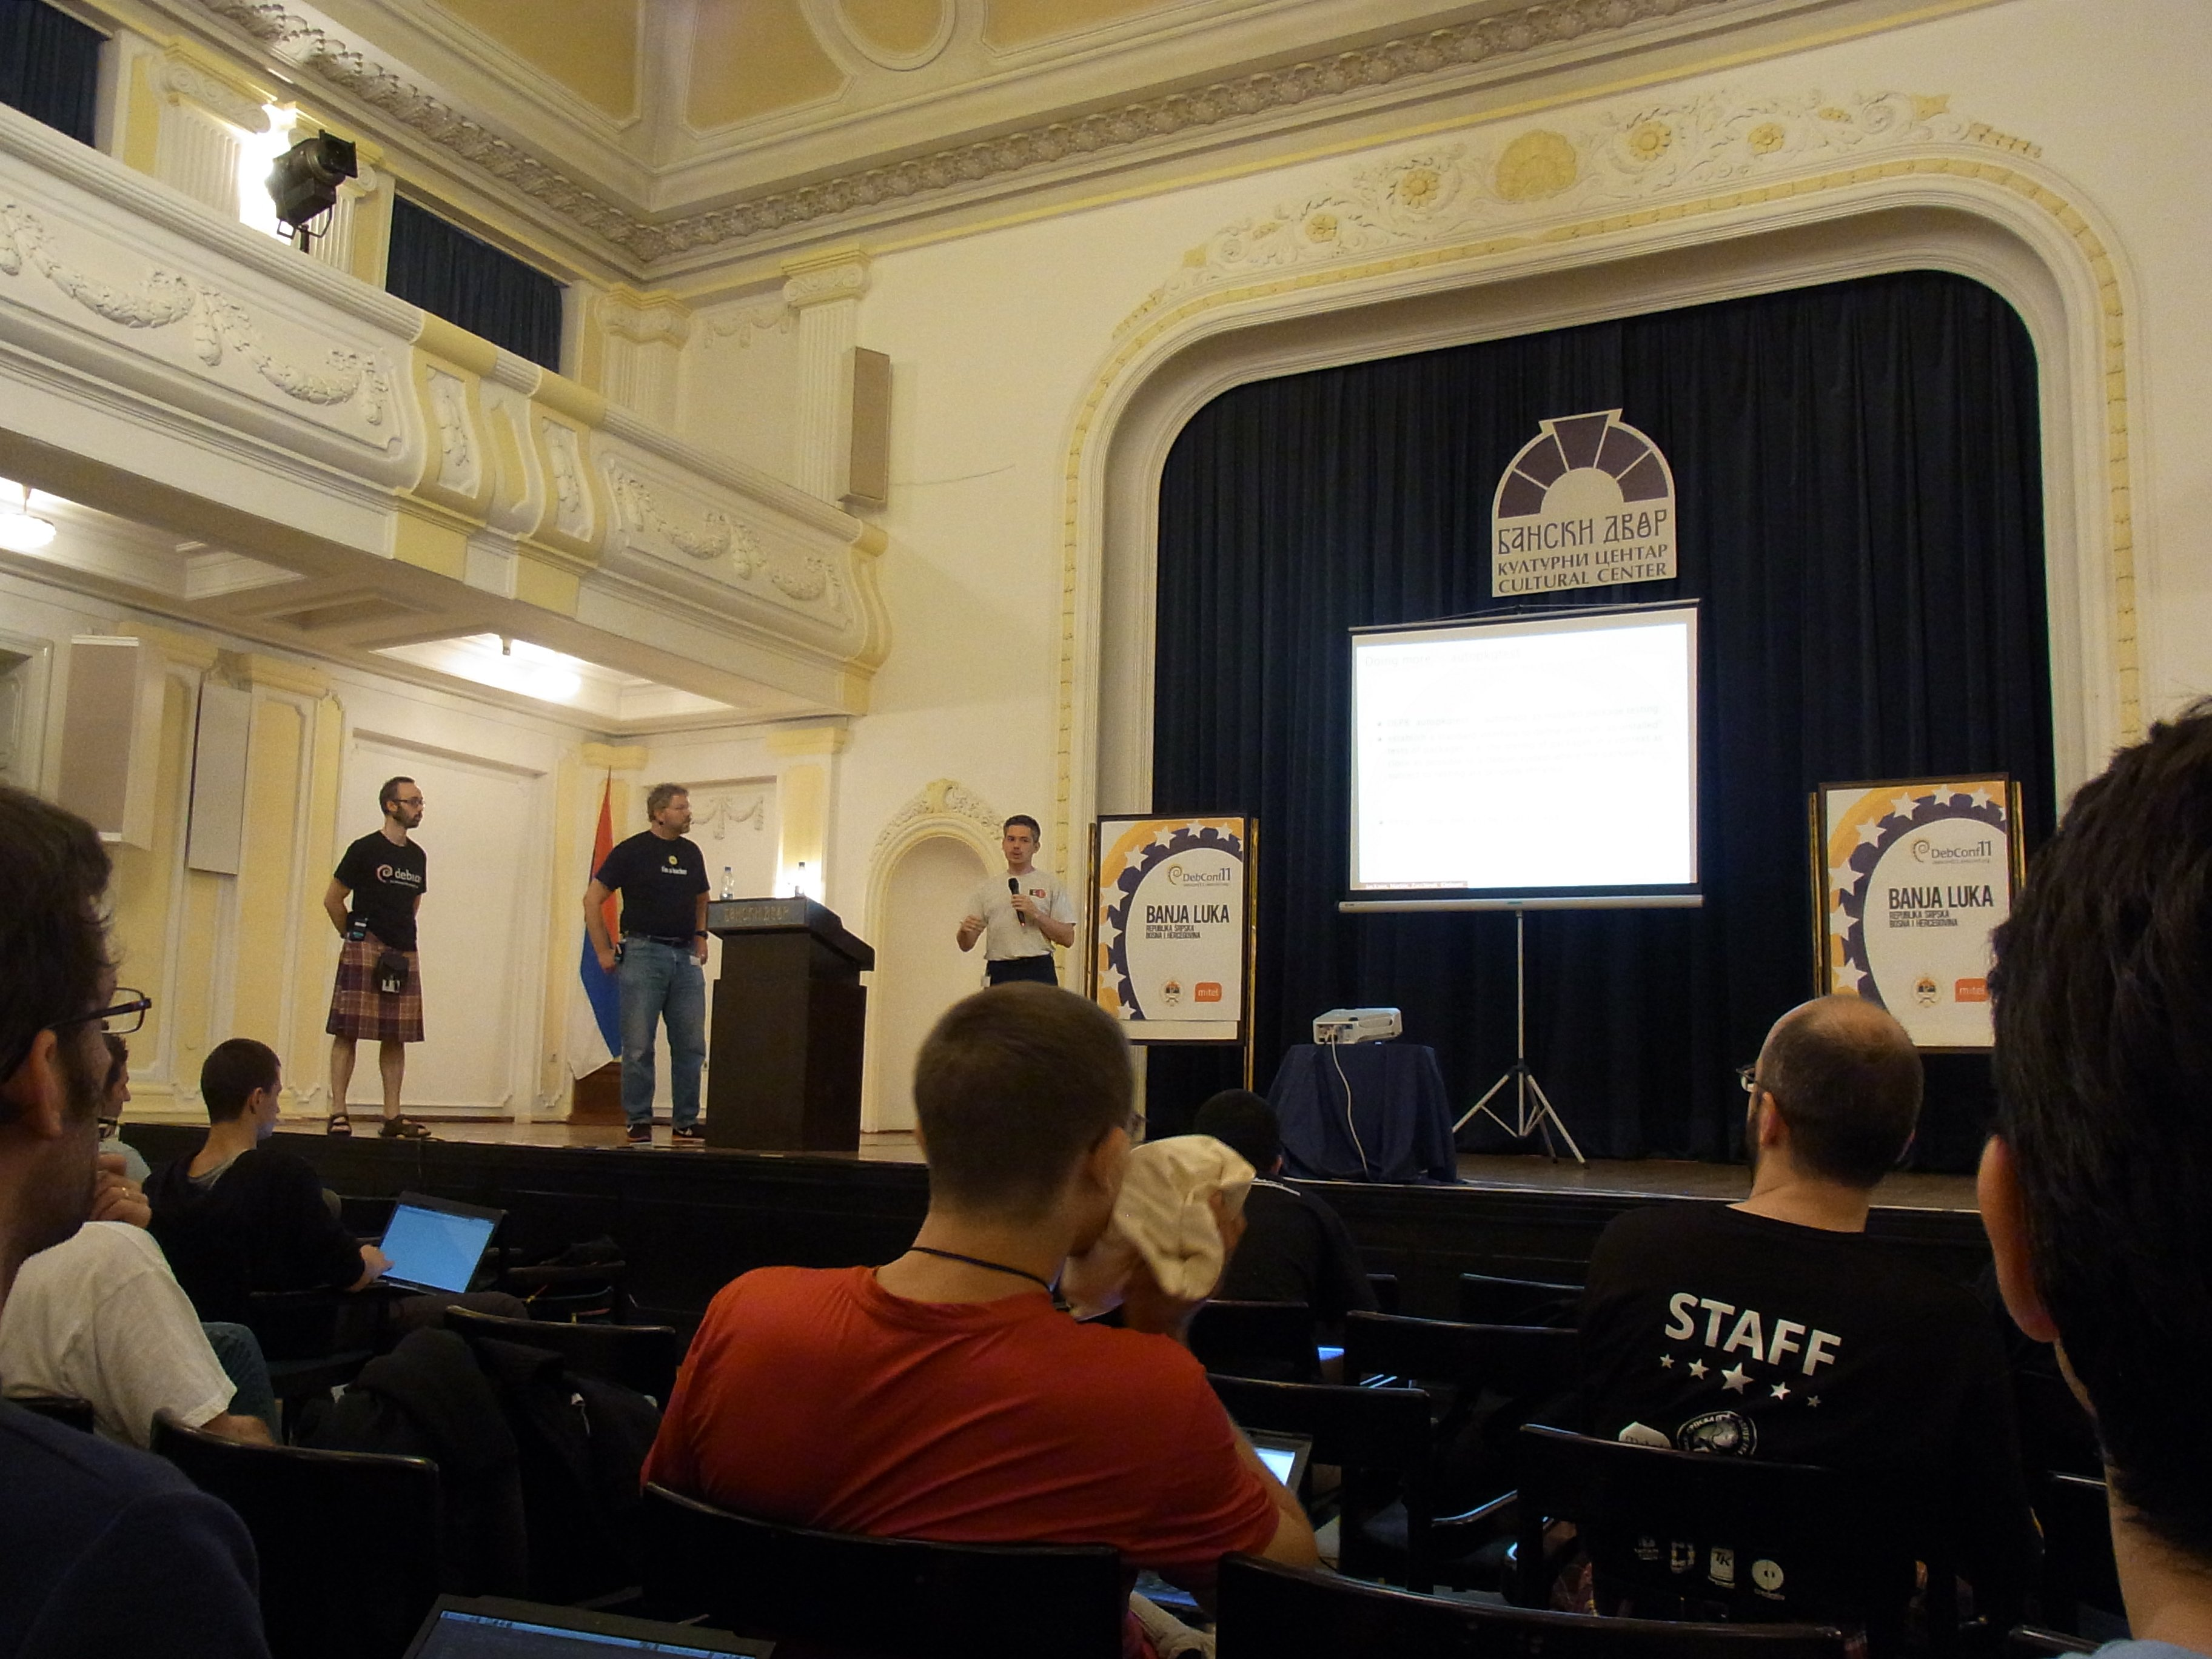
\includegraphics[height=.45\textheight]{./image201108/debconf11_main.jpg}
    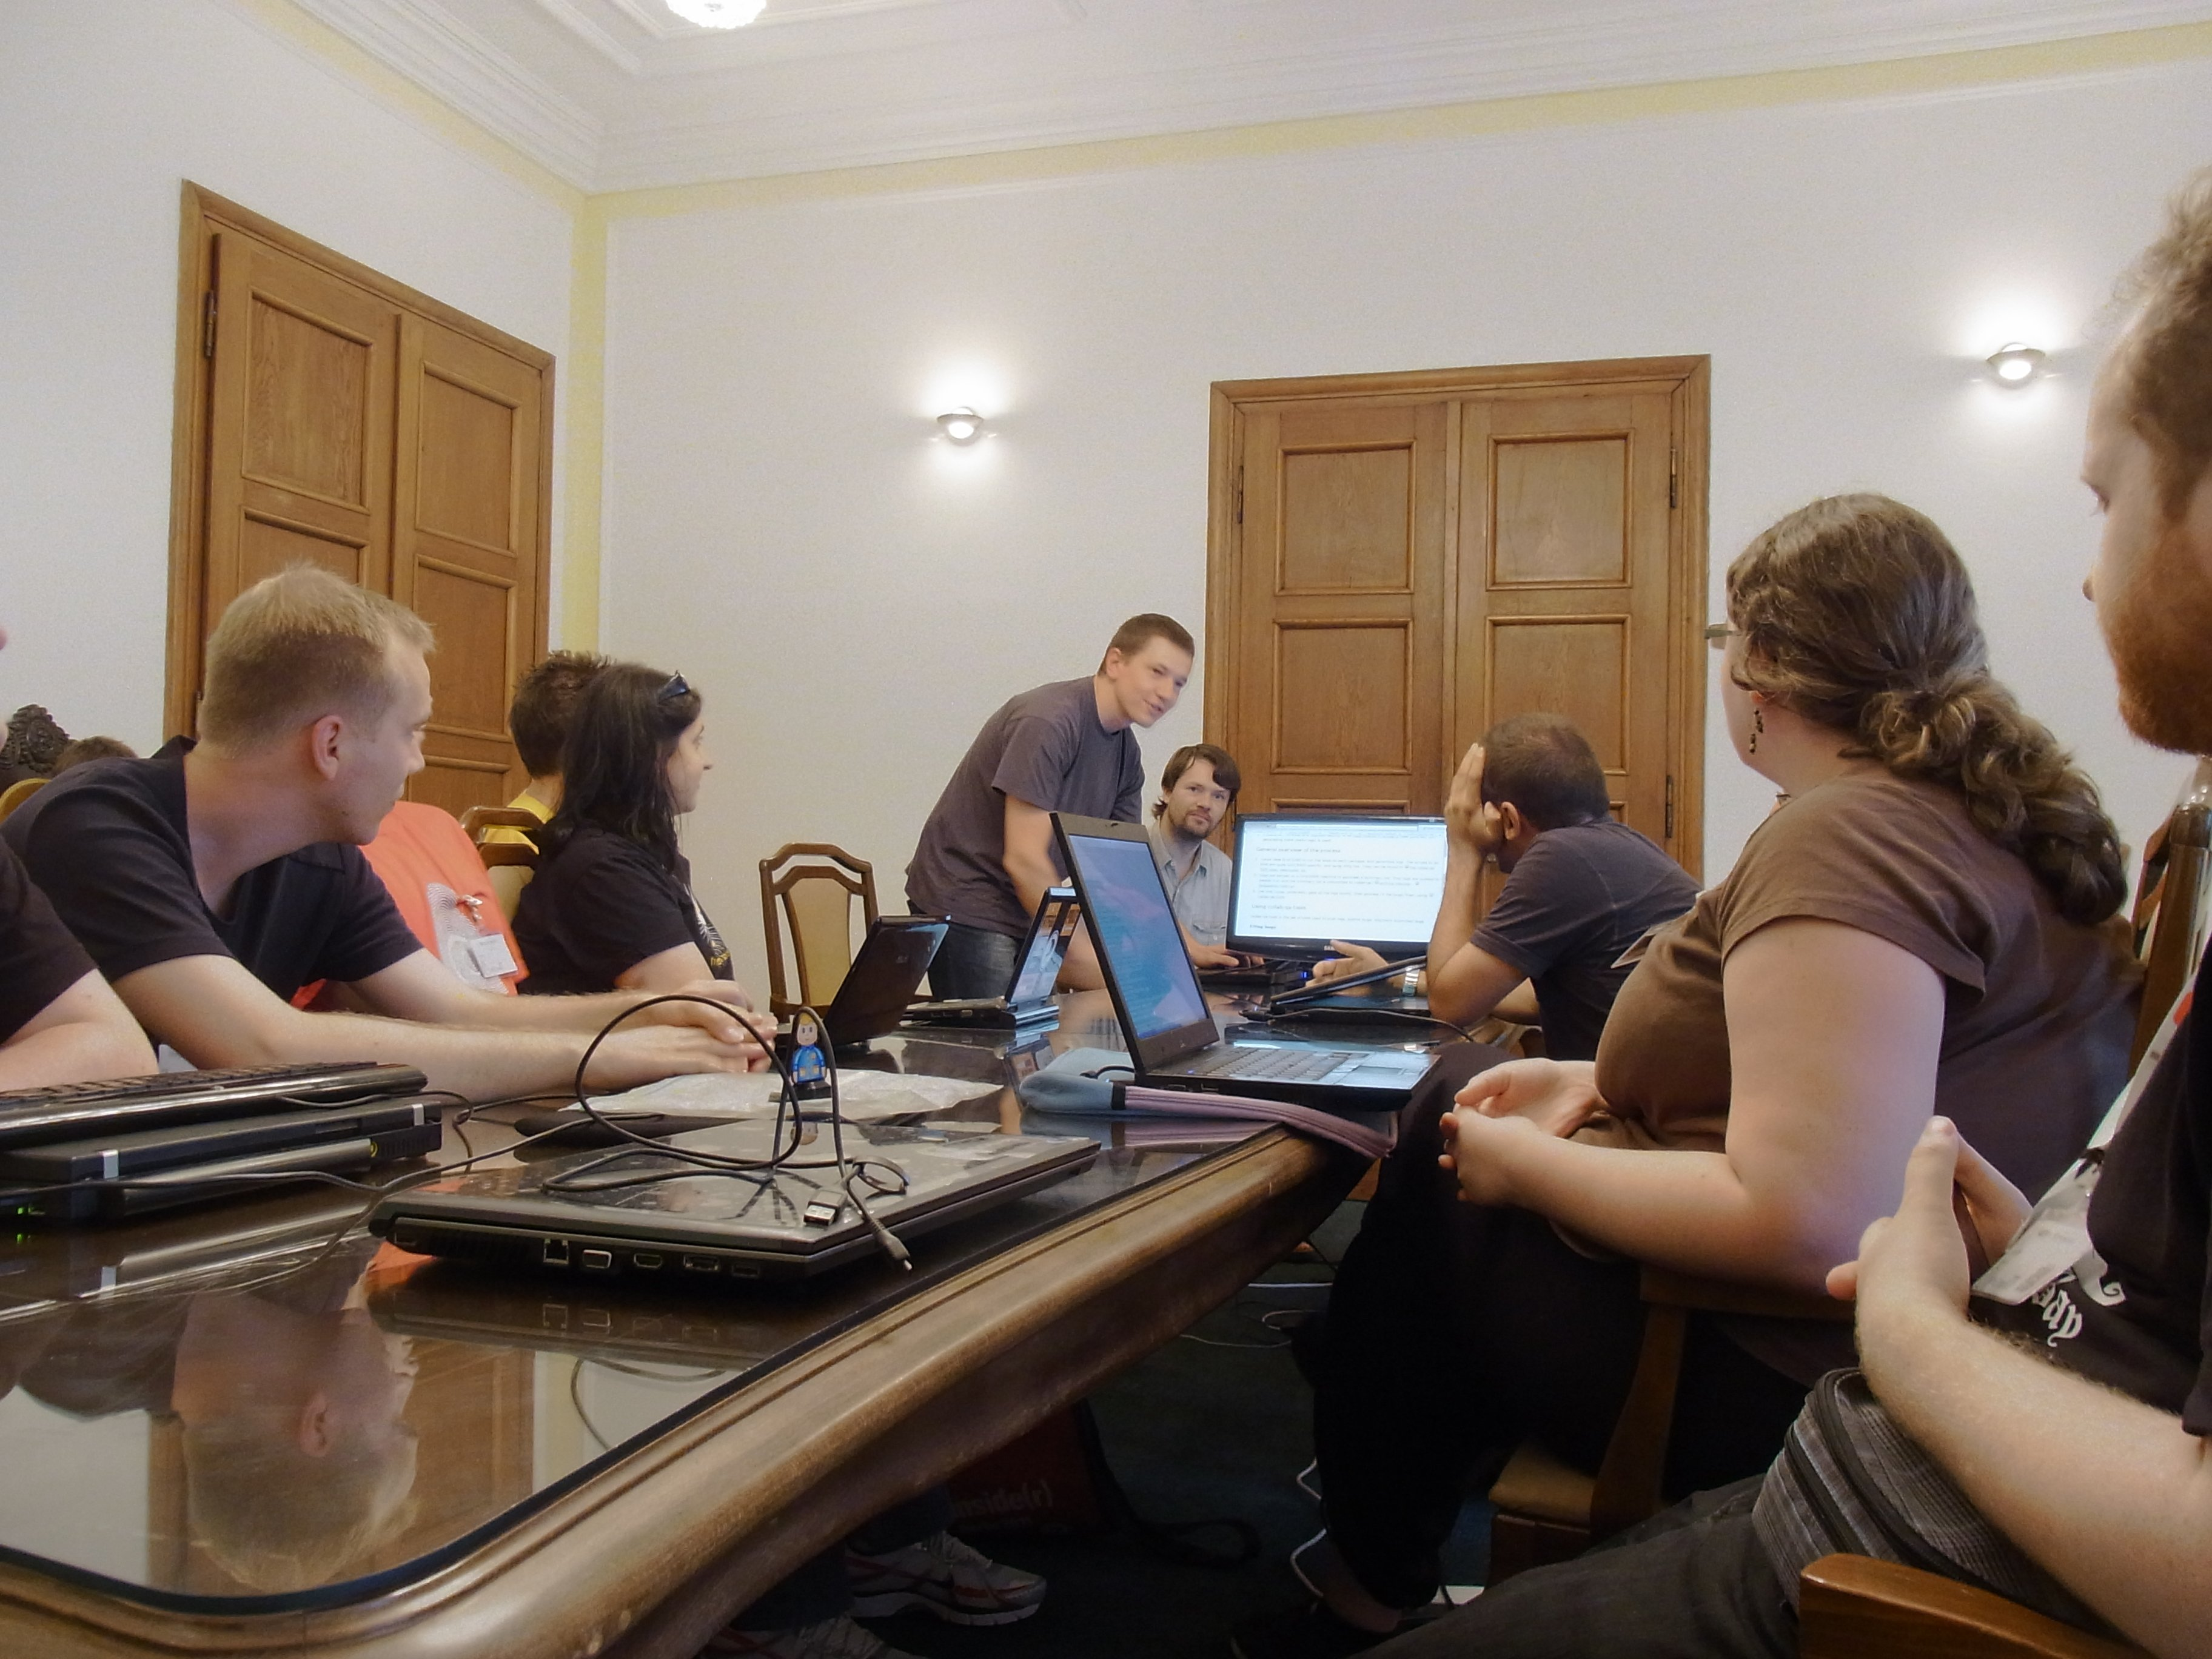
\includegraphics[height=.45\textheight]{./image201108/debconf11_meetingroom.jpg}
  \end{center}
  \centering

\end{frame}

\takahashi[50]{そんな\\こんなで}
\takahashi[120]{次}

\takahashi[50]{事前課題発表}

\begin{frame}[fragile]
\frametitle{事前課題}

\begin{block}{今回の事前課題}
Debian GNU/Linux unstable (sid) が使える環境を用意しておいて下さい。 普段お使いの環境が sid の場合には特に事前課題はありません。普段使いの環境が sid 以外の場合には、以下の方法が考えられます。
\begin{enumerate}

\item VirtualBox などの仮想マシン上に sid を install する
\item (c)debootstrap + schroot で sid 環境へ切り替えられるようにしておく
\item squeeze/wheezy を sid に upgrade する
\end{enumerate}

\end{block}
\end{frame}

\takahashi[50]{参加者の回答\newline 兼自己紹介}

\begin{frame}[fragile]
\frametitle{ のがたじゅん }

普段の環境がsidなので、とくになにもしてません。
\end{frame}

\begin{frame}[fragile]
\frametitle{ 佐々木洋平 }

今更(08/28 08:42) 申し込んでいないことに気がつく愚か者です。

普段から sid 使っています。 schroot もバリバリ。
\begin{commandline}
 $ ls -l /var/chroot
 drwxr-xr-x 22 root root 4096 2011-08-01 08:10 TeXLive-amd64/
 drwxr-xr-x 20 root root 4096 2011-07-14 11:07 lenny-i386/
 drwxr-xr-x 20 root root 4096 2011-07-14 11:07 lenny-amd64/
 drwxr-xr-x 20 root root 4096 2011-05-12 10:07 squeeze-i386/
 drwxr-xr-x 20 root root 4096 2011-05-12 10:07 squeeze-amd64/
 drwxr-xr-x 20 root root 4096 2011-08-14 18:07 sid-i386/
\end{commandline}
%$
\end{frame}

\begin{frame}[fragile]
\frametitle{ 榎真治 }
(無回答)
\end{frame}

\begin{frame}[fragile]
\frametitle{ gdevmjc }
久保です.お世話になります。

2. debootstrap + schroot で sid 環境を作ります。

debootstrap は完了。続いて schroot 勉強中。
\end{frame}

\begin{frame}[fragile]
\frametitle{ 水野源 }

さて、Ubuntu 10.10上にどうやってsid環境作るかね…

\end{frame}

\begin{frame}[fragile]
\frametitle{ murase\_syuka }

(無回答)

\end{frame}

\begin{frame}[fragile]
\frametitle{ かわだてつたろう }

ラップトップでは sid 環境を使っています。
たまーに何かあるようですが、普通に使えています。
\end{frame}

\begin{frame}[fragile]
\frametitle{ ojima.h }

(無回答)

\end{frame}

\begin{frame}[fragile]
\frametitle{ 甲斐正三 }

持参するPCは事情によりSidにできないので、
今回はハンズオン無しでお話を伺うことになると思いますがよろしくお願いします。
(自宅のPCはホスト"amd64-stable"にkvm-qemuでゲスト"i686-sid"を入れています。)

\end{frame}

\begin{frame}[fragile]
\frametitle{ Nao SATO }

debian 歴半年くらいです.普段は squeeze を使っている「なんちゃって」debian ユーザです.26日までには sid を使えるようにはしておくつもりです.

\end{frame}

\begin{frame}[fragile]
\frametitle{ lurdan }

常用環境は sid です。ふつーに使えるよ sid。

\end{frame}

\begin{frame}[fragile]
\frametitle{ kozo2 }

(無回答)

\end{frame}

\begin{frame}[fragile]
\frametitle{ taksaeki }

手元の PC には元々一切 debian 環境がなかったので, パーティションを切り直し, 空いた領域に DVD を使って squeeze をインストールしました.
その後, 3 の方法 (upgrade) をとり, sid が使える環境を構築しました.

\end{frame}

\begin{frame}[fragile]
\frametitle{ sxpxq619@yahoo.co.jp }

2. (c)debootstrap + schroot で sid へ切り替えられるようにする

の方法で, sid 環境を構築しました.

\end{frame}

\begin{frame}[fragile]
\frametitle{ Y.YATSUO }

常用環境をwheezyからsidにdist-upgradeしました。
あっさりアップグレード完了し、今のところ問題無く使えてます。
今までsafe-upgradeするときはあまり内容を吟味せずにyしてしまっていたので今後は気をつけようと思います。

\end{frame}

\begin{frame}[fragile]
\frametitle{ 山田 洋平 }

(c)debootstrap + schroot で sid へ切り替えられるようにして...みます。

\end{frame}

\begin{frame}[fragile]
\frametitle{ よしだともひろ }

ノートPCに 2.(c)debootstrap + schrootでsidへ切り替えるようにしました。

自宅ではVirtualBoxにsidをinstallした環境がありますが、思った以上に普通に使えています。
\end{frame}

\begin{frame}[fragile]
\frametitle{ KAWABATA Takuya }
{\bf{chroot を使ってホーム以下に sid 環境をつくる}}

...以下, ばっさりカット
\end{frame}

\begin{frame}[fragile]
\frametitle{ 川江 }
KVMで仮想マシンにsidをインストールしていいですか?
\end{frame}

\begin{frame}[fragile]
\frametitle{ 山下康成 }
sid ってなんですかぁ???(笑
\end{frame}


\takahashi[50]{そんな\\こんなで}
\takahashi[120]{次}

\section{モダンなDebianパッケージ作成入門}
\takahashi[40]{モダンなDebianパッケージ作成入門\\by 佐々木洋平}

\takahashi[50]{そんな\\こんなで}
\takahashi[120]{次}

\begin{frame}[fragile]
\frametitle{今後の予定(1)}

\begin{block}{第 51 回関西 Debian 勉強会}
  \begin{itemize}
  \item 日時: 9 月 25 日(日)
  \item 会場: 福島区民センター
  \item 内容: 「VCS-buildpackage のお話」
    \begin{itemize}
    \item 講演者: 山下尊也, 佐々木洋平
    \end{itemize}
  \end{itemize}
\end{block}

\end{frame}

\begin{frame}[fragile]
\frametitle{今後の予定(2)}

\begin{block}{KOF 2011}
  \begin{itemize}
  \item 日時: 11 月 11 日(金) -- 12 (土)
  \item 会場: 大阪南港 ATC
  \item 内容: T.B.D.
  \item 講演者: T.B.D
  \end{itemize}
\end{block}

\end{frame}


\takahashi[50]{  }


\end{document}
%%% Local Variables:
%%% mode: japanese-latex
%%% TeX-master: t
%%% End:
